\section{The Web App}

The visualisation of static data has a lot of issues, especially when the data is dynamic. Since the collected data would have needed to be compared to a video to really understand what was going on and what movement hat what effect. Therefore i decided to implement a small web app which will visualise the data in real time. 

This was achieved with a simple C\# MVC website which subscribes to the MQTT broker. Here the switch to MQTT and the extra effort for this switch, was highly beneficial.

The Website started small and was simply used to visualize the collected data:

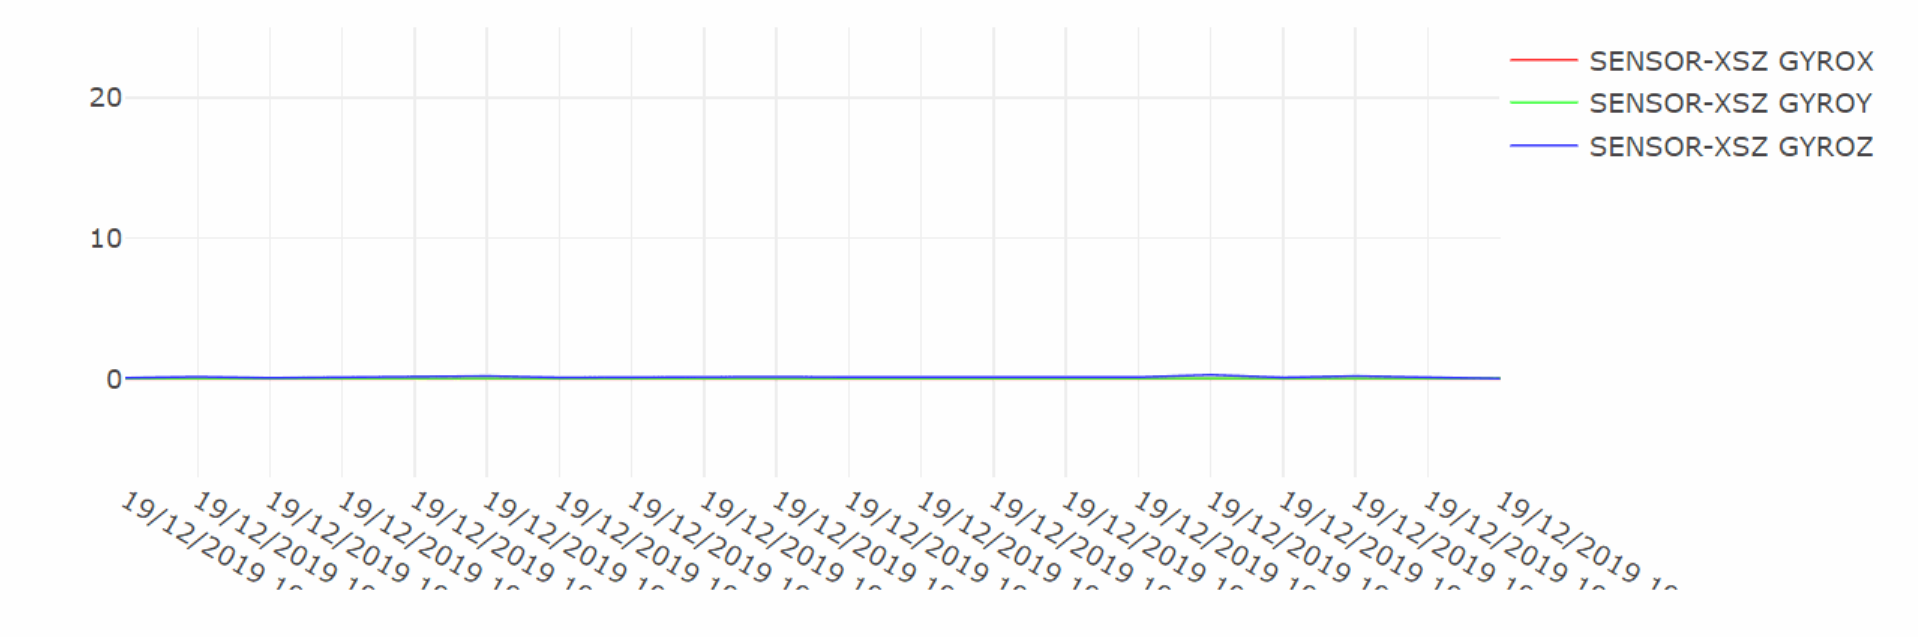
\includegraphics[width=\linewidth]{images/WebVisualisation_SIMPLE.png}

Thanks to this visualisation I was quickly able to understand the data and add additional visualisations and make first conclusions which data was necessary for an in depth analysis. It became clear, that the data needed to be "transferred" into a much more readable format, like pitch, roll and yaw.
The conversion was quite simple and only needs the acceleremoter data:

\begin{lstlisting}
function getRoll(x, y, z) {
    pitch = 180 * Math.atan(x / Math.sqrt(y * y + z * z)) / Math.PI * 4;
    roll = 180 * Math.atan(y / Math.sqrt(x * x + z * z)) / Math.PI * 4;
    yaw = 180 * Math.atan(z / Math.sqrt(x * x + z * z)) / Math.PI * 4;
    return {
        "roll": roll,
        "pitch": pitch,
        "yaw": yaw
    }
}
\end{lstlisting}

With these formula the position of the sensor was really simple to read and visualise and i realised that one sensor would not be enough, since its position does not offer enough information about the posture: 

\begin{figure}[h]
  \begin{center}
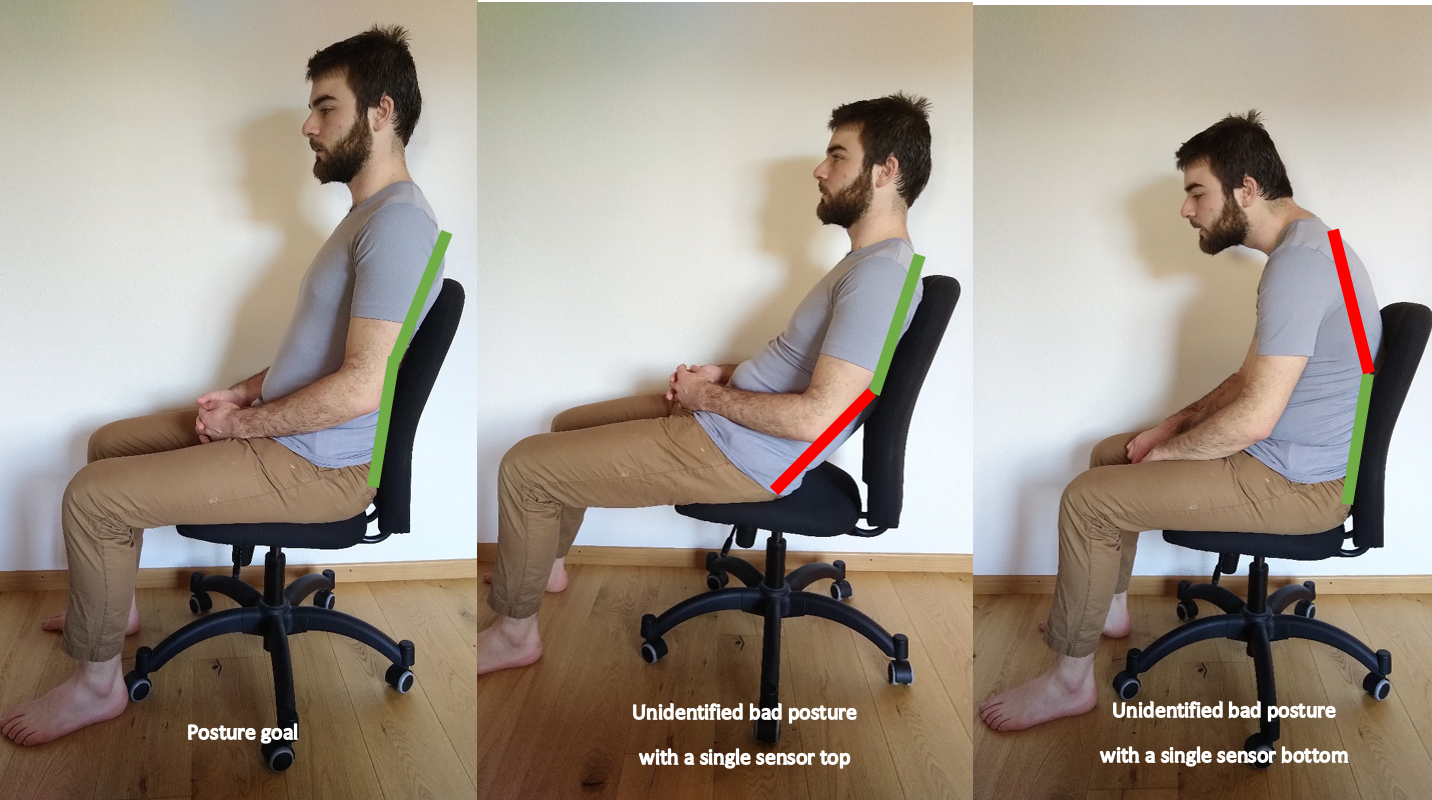
\includegraphics[width=0.3\textwidth]{images/Backposition.png}
  \end{center}
  \caption{Back position}
  \label{fig:BackPos}
\end{figure}

Therefore a minimum of two sensor would definitely be need to make general conclusions from the data. The visualisation was expanded to three to improve the analysis of the data.  The Idea was to calculate the degrees between each sensor to check whether the user has a bent back. This was later overturned, however I might get back to that idea since it would enable the user to have more flexibility when moving, since it would allow for the whole back to move correctly without triggering a warning.

Through the MQTT-Broker the data of three sensors is sent as JSON. In the JSON is the UID of the sensor with which it is identified. Then the data is parsed and passed through a javascript library (plot.ly) \cite{ModernAn18:online} to create the graphs. To simplify the analysis of the data i further also knew the position of each sensor:

\begin{figure}[h]
  \begin{center}
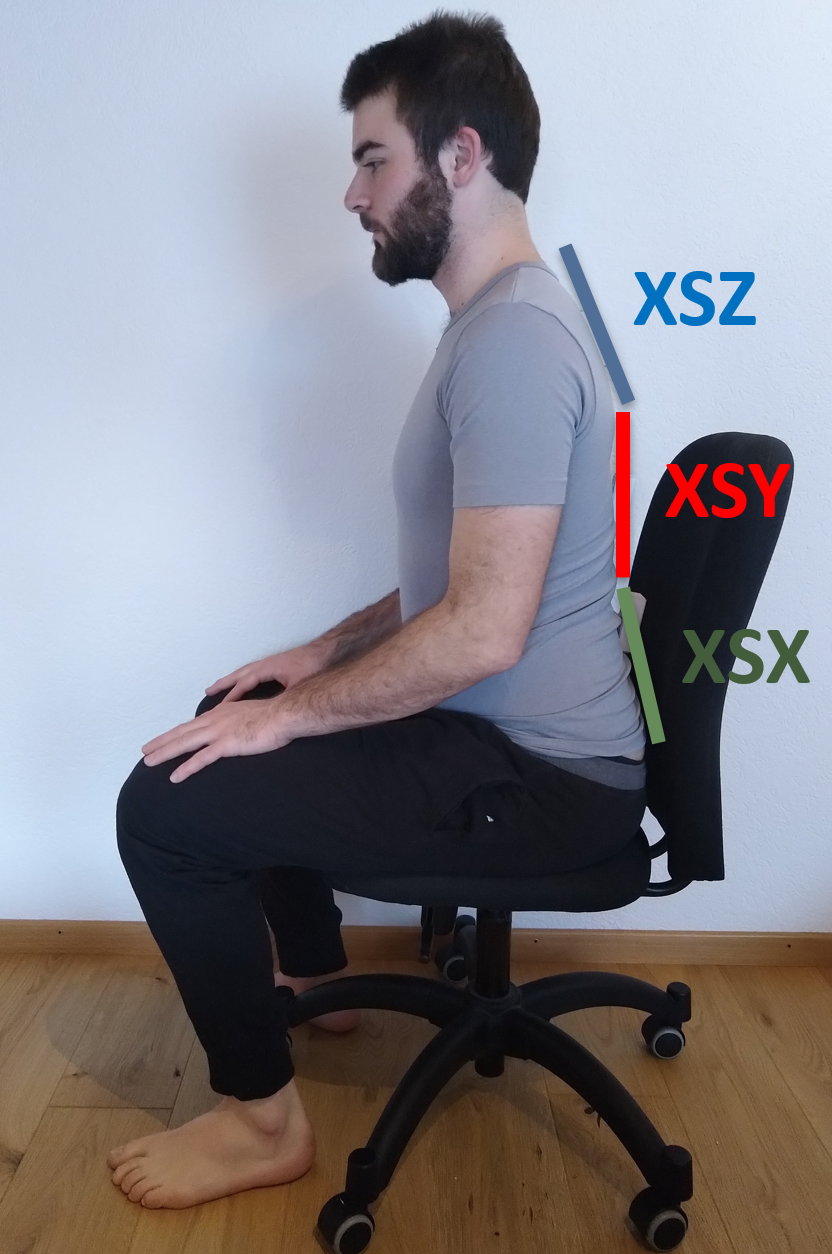
\includegraphics[width=0.3\textwidth]{images/ChairVisualised.png}
  \end{center}
  \caption{Sensor position}
  \label{fig:BackPos}
\end{figure}

After some research, testing and discussion with a physiotherapist, we realised, that the approach of trying to set a general goal for all users was not correct, in many ways. Different studies found that posture is a very individual thing and cannot be set globally \cite{SitUpSt77:online} therefore we decided to implement functionality so that each user can set his/her own individual goals. I will get further into these decision in the \ref{chap:Results}.

\subsection{Functionality}

Thanks to this setup, the web app could not only be used to visualise the data but also to add functionality and use this live data to help the user improve his/her posture. This was achieved with two, lets call them, modes. 

The first mode is the "Goal" mode, where the user can set a goal posture which he would like to achieve and keep. The user clicks to button "calibrate" and then the desired posture needs to be held for at least 10 seconds. 
Now every sensor has a calibrated optimal value. Each deviation of this optimal value is visualised, and when a threshold is reached a warning is triggered to the user. In the beginning of this project the warning was only visual, however a tactical feedback from the sensor itself was implemented later on.

These modes are visualised as below. In the circle you see a red line and a green line. Here the avoid mode is visualised where the red line is the position the user would like to avoid and the green line is his current position.

\begin{figure}[h]
  \begin{center}
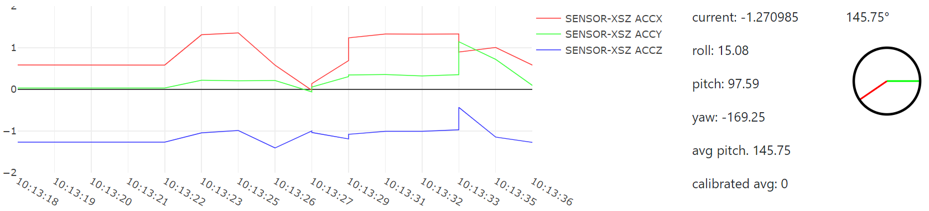
\includegraphics[width=\textwidth]{images/WebAppCircle.png}
  \end{center}
  \caption{Target position}
  \label{fig:BackPos}
\end{figure}

The second mode is very similar, however a position the user would like to avoid is programmed and the sensor react when the user gets to close to this position rather than to far away. 

For the calculation of these modes each sensor was only analysed individually, however this could be easily improved by calculating the overall changes of position, so to accumulate each sensors deviation, in degrees. This would enable the web app to trigger a warning when the user is bent to much or too little.

